\section{Task1: Implementation of NeRF accelerate method}
\label{sec:intro}

We took $3$ videos in different scenarios, then we can implement the dataloader of them, and put them into the vinilla NeRF, the NGP, and the TensoRF. Then we could compare the difference among them.

% --------------------------------
\subsection{Scenarios}
\label{scenarios}

To make the testing diverse, the scenarios were taken indoor and outdoor, big and small.

The scenario $1$ is a small object stationery.

The scenario $2$ is a bigger object chair.

The scenario $3$ is also a chair, but with matting preparation in order to chase for a better behavior. The code part for the matting can be seen in to folder '\textit{matting tool'}. 

The $3$ scenarios look like in figure \ref{the 3 scenarios}. From left to right are scenario $1$, scenario $2$, scenario $3$ respectively.

\begin{figure}[htbp]
	\centering
	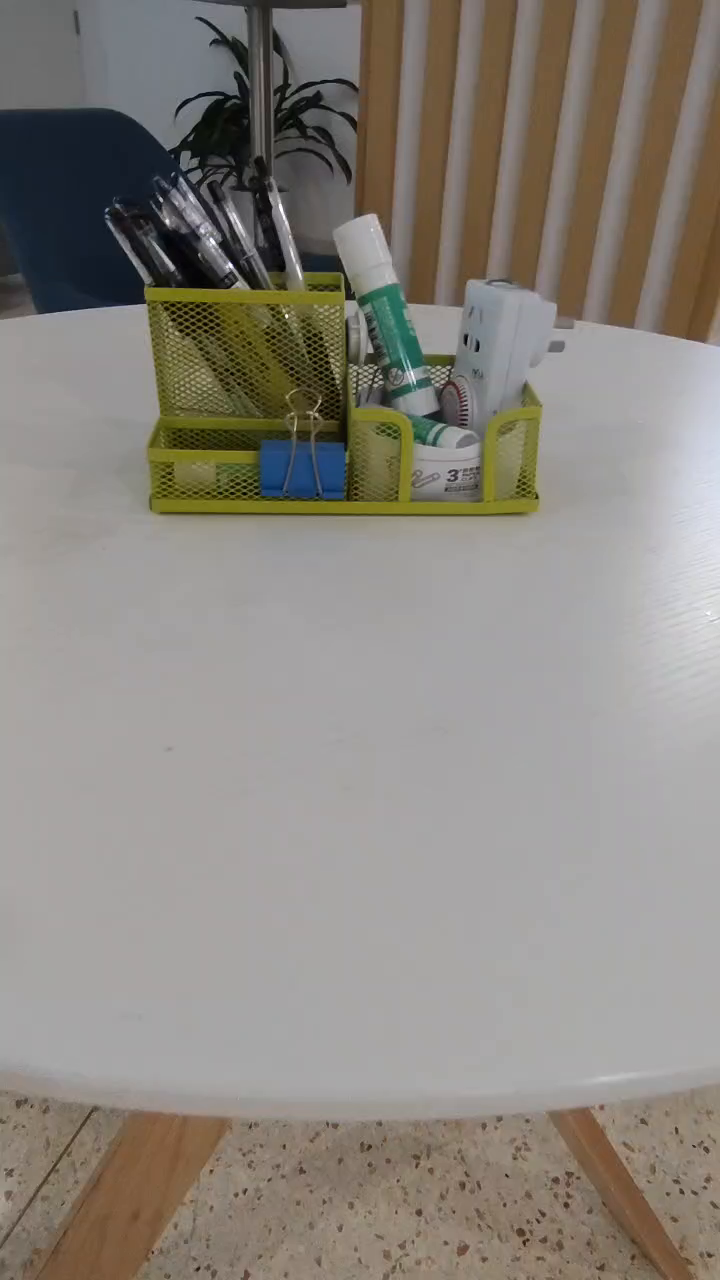
\includegraphics[width=0.32\linewidth]{result/scenario/scenario1.png}
	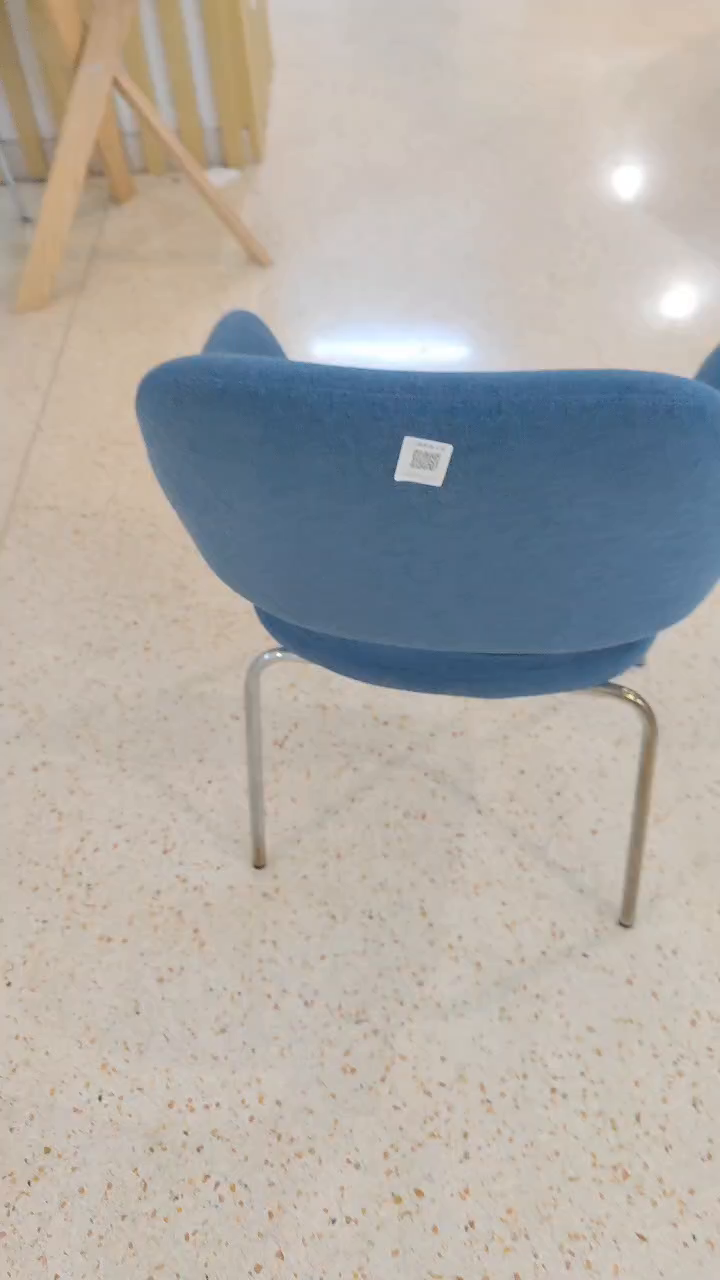
\includegraphics[width=0.32\linewidth]{result/scenario/scenario2.png}
	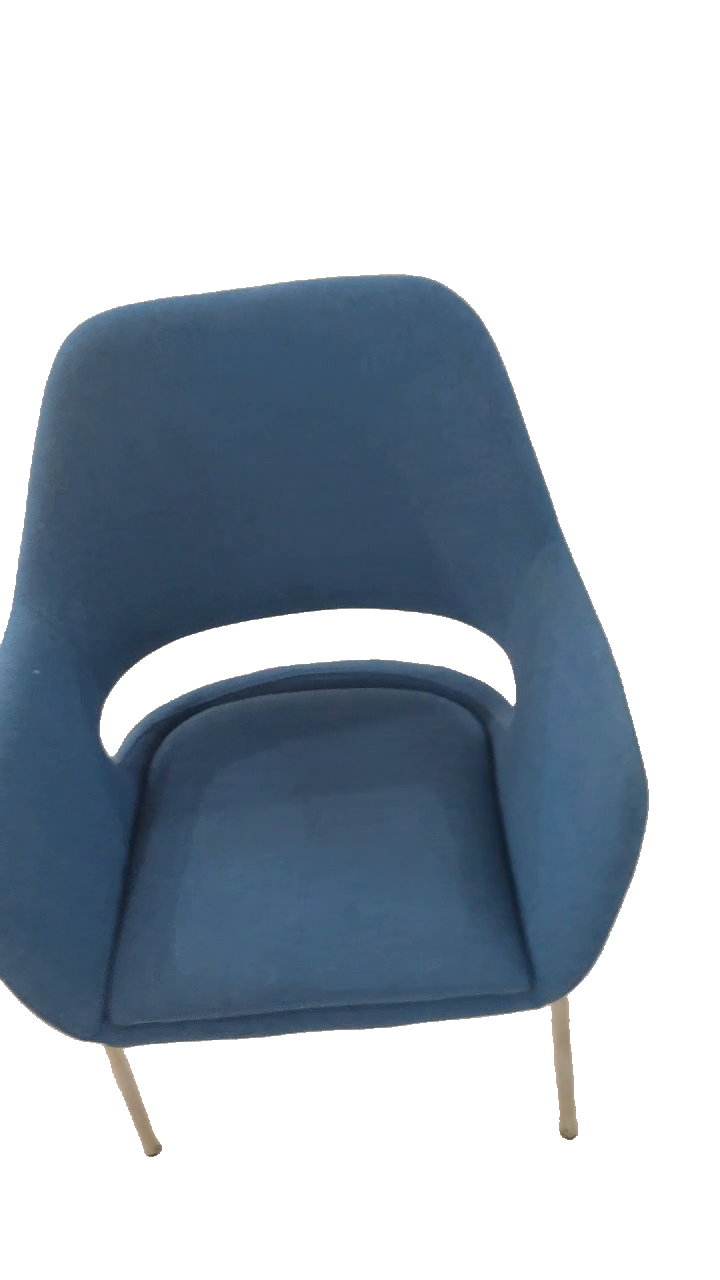
\includegraphics[width=0.32\linewidth]{result/scenario/scenario3.png}
 \caption{the $3$ scenarios}
	\label{the 3 scenarios}
\end{figure}

% --------------------------------
\subsection{dataloader}
\label{data loader}

Since we took the videos of the $3$ scenarios, but the NeRFs' input should be the images and the intrinsic parameters of the cameras.

With the help of the nerfstudio's integration, and the usage of colmap, we can input the video, and generate the internal and external parameters of cameras. Which is exactly the input for NeRF.

And the frames of the videos were split into the training dataset, validation dataset, and the testing dataset. Each dataset include the images and the correspondence cameras' intrinsic parameters.

Then with the prepared datasets, we could implement the methods in different scenarios.

%  --------------------------------
\subsection{metrics}
\label{metric}
The training information training time(minute:second),  GPU memory consumption(MB), and the training  metrics are PSNR, SSIM, LPIPS. The methods' metrics comparison are shown in the section \ref{conclusion}.

Where PSNR, SSIM and LPIPS are metrics to evaluate image quality.

- PSNR(Peak Signal-to-Noise Ratio) is defined as:
$$\text{PSNR}=10\cdot \log_{10}\dfrac{\text{MAX}_I^2}{\text{MSE}}$$
Where $\text{MAX}_I$ is the max value of the pixels in image $I$, and the MSE of two images $I,K$ is:
$$\text{MSE}=\dfrac{1}{mn}\sum_{i=0}^{m-1}\sum_{i=0}^{n-1}\|I(i,j)-K(i,j)\|^2$$

- SSIM(Structural Similarity Index Measure) is used for comparing the similarity of two images from $3$ key features: Luminance, Contrast, and Structure.

1. Luminance is the average gray scale measurement, obtained by averaging the values of all pixels. Defined as:
$$\mu_x=\frac{1}{N} \sum_{i=1}^N x_i$$
And its contrast function is:
$$l(x, y)=\frac{2 \mu_x \mu_y+C_1}{\mu_x^2+\mu_y^2+C_1}$$

2. Contrast is easured by the grayscale standard deviation. Unbiased estimation of standard deviation:
$$\sigma_x=\left(\frac{1}{N-1} \sum_{i=1}^N\left(x_i-\mu_x\right)^2\right)^{\frac{1}{2}}$$

And its contrast function is:
$$c(x, y)=\frac{2 \sigma_z \sigma_y+C_2}{\sigma_z^2+\sigma_y^2+C_2}$$

3. Structure is the comparison is made after normalization $x-\dfrac{\mu_x}{\sigma_x}$ and $\dfrac{y-\mu_y}{\sigma_y}$, i.e. can be measured by correlation coefficient:

$$s(x, y)=\frac{\sigma_{x y}+C_3}{\sigma_x \sigma_y+C_3}$$
$$\sigma_{x y}=\frac{1}{N-1} \sum_{i=1}^N\left(x_i-\mu_x\right)\left(y_i-\mu_y\right)$$

So SSIM is the combination of Luminance, Contrast, and Structure:
$$\text{SSIM}(x, y)=l(x, y)^\alpha \cdot c(x, y)^\beta \cdot s(x, y)^\gamma$$
Where $\alpha, \beta, \gamma$ is the ratio of each of the $3$ parts of the features.

- LPIPS(Learned Perceptual Image Patch Similarity)  is an indicator for measuring image similarity. It learns an image similarity measurement method through deep learning that can better simulate the human visual system.  The lower it is, the two images are more likely to be the same.